\chapter{Deep Learning Models for Fetal Pain Assessment}

% In this chapter, we present some background topics recommended for a better understanding of our work and later explain the methodology that was used to conduct our experiments.

% \section{Methodology}

Based on the techniques mentioned in Chapter 3, we have proposed a learning model for classifying between images of fetuses with facial expressions indicative of pain or not. In summary, our proposed pipeline consists of sampling the videos into frames, finding the images which contain a clear fetus face, and training a CNN in with the binary classification task of finding the presence of pain. In the following sections, we describe each of these steps.

\section{Image Sampling}

It is common to have a small number of data to work within the medical field, given the inherent difficulty of collecting it. In our case, especially, only a small percentage of pregnancies require intra-uterus intervention before birth, and thus fetal anesthesia is a relatively rare procedure. 

Thus, we ended up with 15 videos available. However, it is relatively common for studies in the field to also have a small N, as mentioned by \cite{ZamzmiPGKSA16}.

Since we had such a small number of videos, it was not possible to work with them directly. So, we decided to bring the data to another dimension, reducing the space from videos to images. In order to do this, we decided to sample the videos and capture frames at a rate of 2 seconds. 

With this process, we generated a total of 708 images, but since the images were recorded from ultrasound machines, they depend on the calibration by the doctors to capture the exact section of the 3-D space where the fetus's face is clear. Because of this, it was common to find parts of the video where the face of the fetus was not visible and showed non-distinguishable parts.

As we had a significant number of images, and manual selection would be not only hard but also dependent on the observant, this became a problem.

To overcome this issue, we decided to use another neural network capable of detecting facial landmarks, like the nose, the mouth, and the eyes. The network we used was the Multi-task Cascaded Convolutional Networks (MTCNN) developed by \cite{ZhangZL016}, which identifies faces in images. It worked surprisingly well in our domain, even though the images had quite different characteristics.

With this process, we were able to filter out our dataset of images from 708 to 357 and be sure the images contained a clear face. The network returns a confidence number of which it found the face in the image, and we have used only confidences of over 95\%, which on manual inspection showed to be very reliable, with just six clear errors that were removed manually.

The position of the facial landmarks allowed us to crop the images around the face of the fetus, which is done just by adding padding to the places where they were. This process is achievable after we have the positions of the landmarks returned through the MTCNN, which also makes face alignment possible. This helps to discard images with blurred surroundings around the fetus, which contains non-distinguishable parts.  Figure \ref{fig:cropping} shows an example of a cropped image.

\begin{figure}[h!tp]
    \centering
    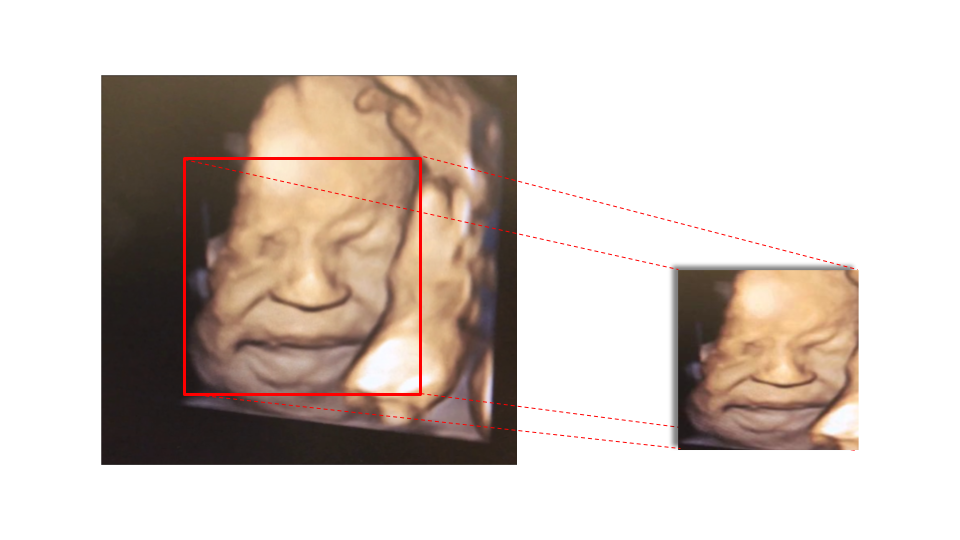
\includegraphics[width=.9\textwidth]{imgs/chap5_cropping.png}
    \caption{Image cropping with MTCNN}
    \label{fig:cropping}
\end{figure}

At this point, manual selection was needed in other to separate the images back into the three groups. With the resting images, it was easy as all the frames were from resting positions. However, with the anesthesia and horn ones, we had to split the data between before and after the stimulus. This was not a complicated process as we knew precisely when the stimuli were applied, and a clear difference in the facial expression could be noted.

\section{Data Augmentation}

Even though we had increased the size of the dataset by turning the videos into images, it is still considered a relatively small dataset for deep learning models. To further augment our chances of succeeding, we have applied the use of data augmentation techniques to increase the variability of our data. The effectiveness of this technique has been demonstrated by \cite{abs-1712-04621} and is widely used in the field.

There is a wide variety of transformations possible for using data augmentation, and the most straightforward ones usually work very well. We have chosen the following:

\begin{itemize}
    \item Horizontal flip, which consists of mirroring the image horizontally. 
    \item Rotation, which consists in applying small rotations to the images.
    \item Zoom, which consists of zooming in the image.
    \item Lightning, which consists of changing the brightness and the contrast of the image.
    \item Warping, which consists of adding distortions to the image. 
\end{itemize}

All of these methods have a probability of being applied and can be used in combination with each other. Thus for each image, given the probability, a combination of these techniques would be applied. Some examples of these different combinations within the same image are shown in Figure \ref{fig:data_augmentation}.

\begin{figure}[h!tp]
    \centering
    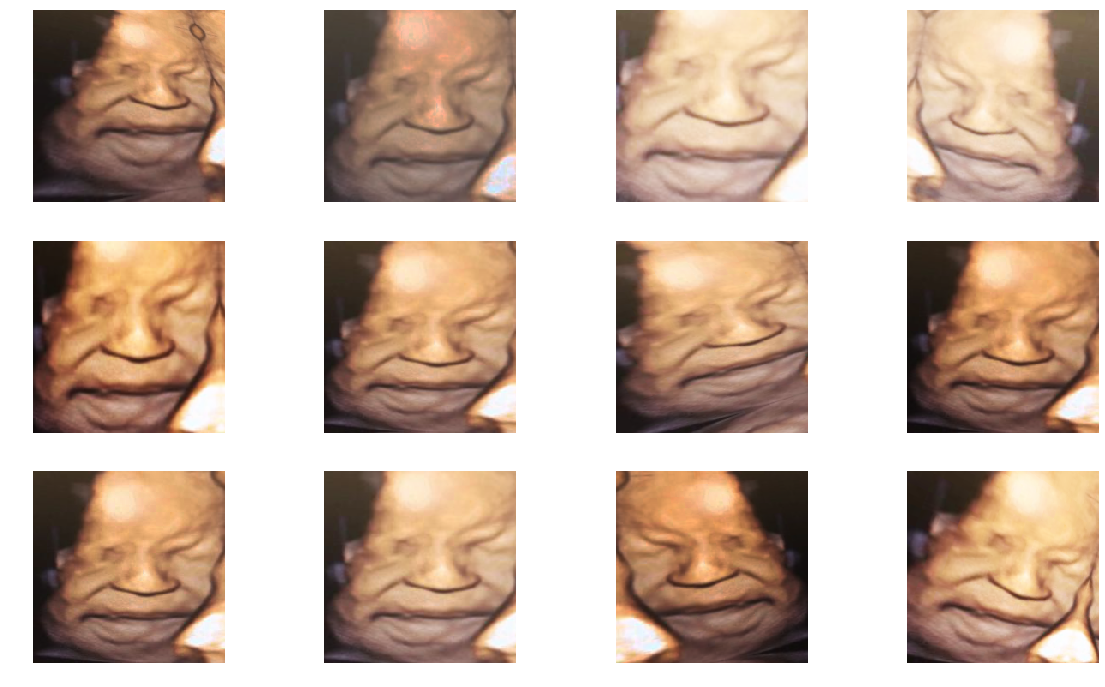
\includegraphics[width=.9\textwidth]{imgs/chap5_data_augmentation.png}
    \caption{Application of different data transformations to a fetus image}
    \label{fig:data_augmentation}
\end{figure}

To further experiment with this process, we have compared three levels of intensity in the changes, a smooth one, which does more subtle changes, a medium one, which intensifies a little bit and a more aggressive one, which applies substantial transformations to the images.

\section{Residual Networks}

The network used was a ResNet created by \cite{ParkhiVZ15}.

\section{Transfer Learning}

VGGFace2: \citep{Cao2018}

ImageNet: \citep{DengDSLL009}


% The loss function we used was binary cross-entropy, as it shows good performance for classification problems with two classes. This loss function is given by the following formula:

% where λ is the set of weights, n is the number of samples in the batch, yi is the true output of the ith patient, pi is the predicted output for the ith patient, and k is the number of neurons to regularize. We optimize the network weights using Adam [Kingma and Ba, 2014], a stochastic optimization method with adaptive momentum, that is able to quickly achieve low error on the training set.


